\documentclass[tikz,border=6pt]{standalone}
\usepackage[scaled]{helvet}
\renewcommand{\familydefault}{\sfdefault}
\usetikzlibrary{arrows.meta,positioning,fit,calc}
\definecolor{ink}{HTML}{12343B}\definecolor{chill}{HTML}{2B7A9E}\definecolor{ice}{HTML}{DCEBF1}
\definecolor{mint}{HTML}{DDEFE7}\definecolor{sand}{HTML}{F5EBCF}\definecolor{grey}{HTML}{EEF3F4}
\tikzset{
 box/.style={draw=ink,rounded corners=2pt,align=center,font=\small,minimum height=10mm,text width=33mm,inner sep=3pt},
 src/.style={box,fill=grey}, proc/.style={box,fill=ice}, res/.style={box,fill=mint}, ctx/.style={box,fill=sand},
 arr/.style={-{Stealth[length=2.4mm]},draw=ink,thick}, head/.style={font=\small\bfseries,text=ink}}
\begin{document}
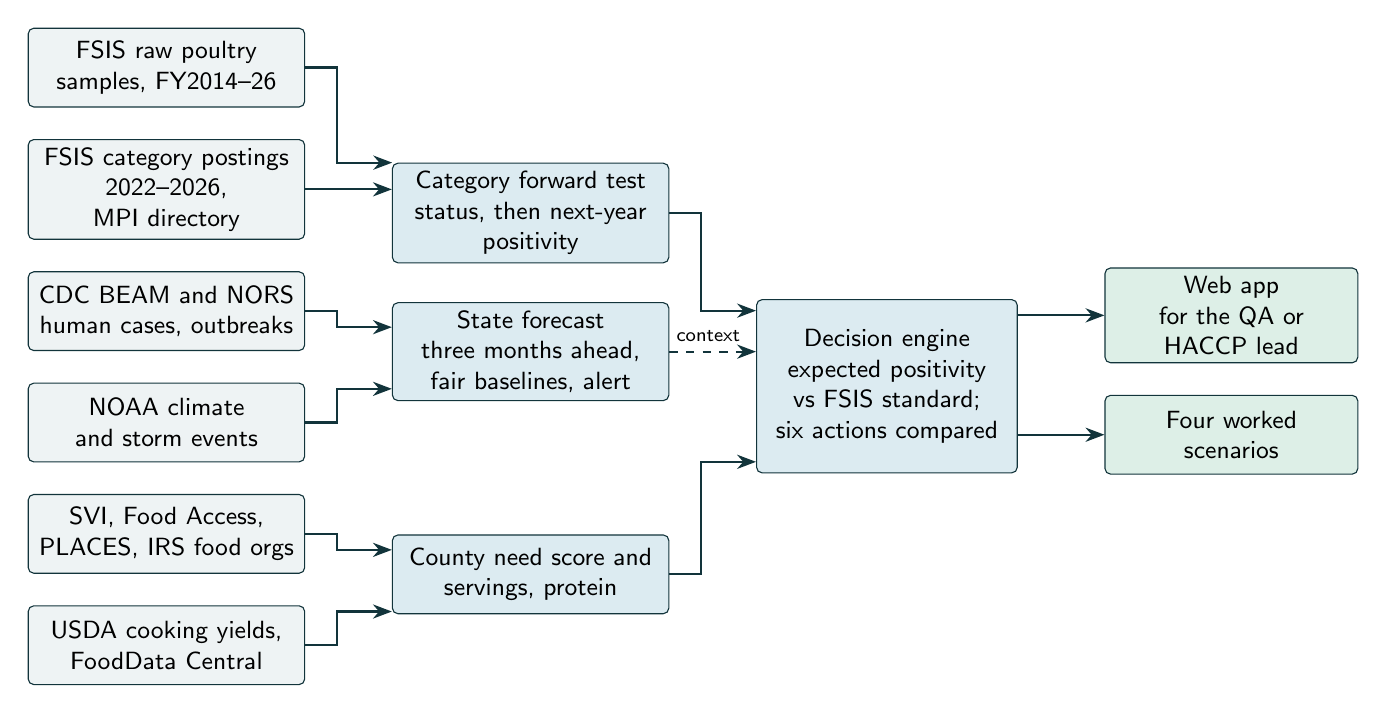
\begin{tikzpicture}[node distance=4mm and 11mm]
\node[src] (fsis) {FSIS raw poultry\\samples, FY2014--26};
\node[src,below=of fsis] (cat) {FSIS category postings\\2022--2026, MPI directory};
\node[src,below=of cat] (beam) {CDC BEAM and NORS\\human cases, outbreaks};
\node[src,below=of beam] (noaa) {NOAA climate\\and storm events};
\node[src,below=of noaa] (need) {SVI, Food Access,\\PLACES, IRS food orgs};
\node[src,below=of need] (nut) {USDA cooking yields,\\FoodData Central};
\node[proc,right=of cat,yshift=-3mm] (forward) {Category forward test\\status, then next-year\\positivity};
\node[proc,right=of noaa,yshift=9mm] (fc) {State forecast\\three months ahead,\\fair baselines, alert};
\node[proc,right=of nut,yshift=9mm] (county) {County need score and\\servings, protein};
\node[proc,right=of forward,yshift=-22mm,text width=31mm,minimum height=22mm] (eng) {Decision engine\\expected positivity\\vs FSIS standard;\\six actions compared};
\node[res,right=of eng,yshift=9mm,text width=30mm] (app) {Web app\\for the QA or\\HACCP lead};
\node[res,below=of app,text width=30mm] (scen) {Four worked\\scenarios};
\draw[arr] (fsis.east) -- ++(4mm,0) |- (forward.160);
\draw[arr] (cat.east) -- (forward.west |- cat.east);
\draw[arr] (beam.east) -- ++(4mm,0) |- (fc.170);
\draw[arr] (noaa.east) -- ++(4mm,0) |- (fc.195);
\draw[arr] (need.east) -- ++(4mm,0) |- (county.170);
\draw[arr] (nut.east) -- ++(4mm,0) |- (county.195);
\draw[arr] (forward.east) -- ++(4mm,0) |- (eng.150);
\draw[arr,dashed] (fc.east) -- node[above,font=\scriptsize,pos=.45]{context} (eng.west |- fc.east);
\draw[arr] (county.east) -- ++(4mm,0) |- (eng.210);
\draw[arr] (eng.east |- app.west) -- (app.west);
\draw[arr] (eng.east |- scen.west) -- (scen.west);
\end{tikzpicture}
\end{document}
